\chapter{Introduction}
Todo.

\textbf{From RAS2023:}

Humanoid robots, thanks to their ability to perform legged locomotion,
are in principle capable of moving through 3D environments, for which complex
motions might be required. These can include stepping over or onto obstacles,
climbing and descending stairs, moving through surfaces located at different
height, overcoming gaps, and so on.

Walking on uneven ground, however, is a challenging task. Management of the
footstep locations is subject to several constraints that are completely absent
in flat ground locomotion, such as the necessity to avoid placing the feet over
the edge of a stair step, or determining whether a given feature of the
environment should be considered useful surface onto which the robot can
step or simply regarded as an obstacle and avoided altogether.

Also from a control standpoint, walking on uneven ground introduces
complications in the dynamic model that are not present in flat ground
locomotion. In fact, traditional humanoid locomotion is realized by
approximating the dynamics using linear models, which are relatively accurate
in many application. Straight up extending these models to 3D environments can
lead, without additional considerations, to nonlinearities which can severely
impact the performance and theoretical guarantees of the controller.

\begin{figure}
    \centering
    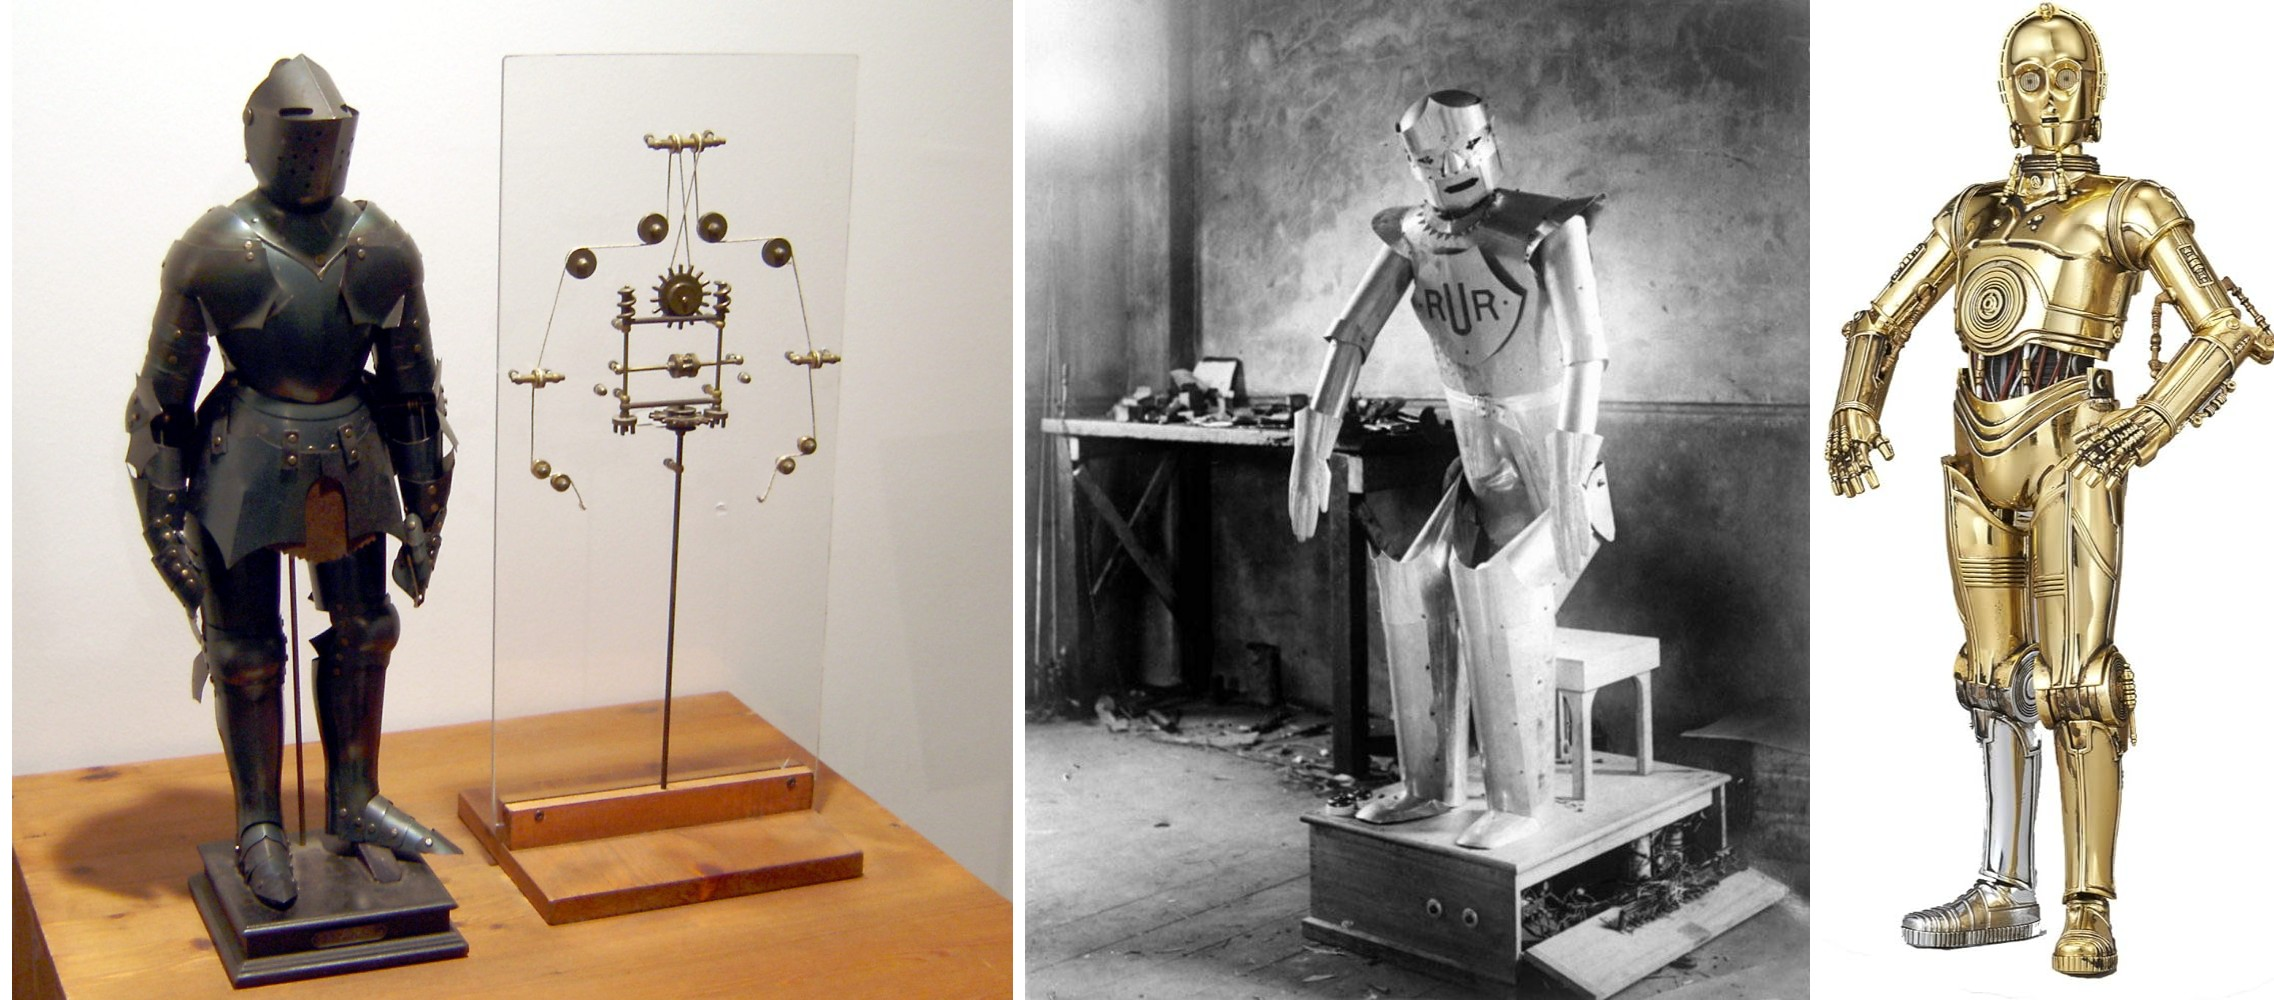
\includegraphics[width=\textwidth]{figures/01-introduction/robot-history.jpg}
    \caption{The Da Vinci robot \cite{Moran2006TheDaVinciRobot}.
        Rossum's Universal Robots \cite{Capek1920RUR}.
        C-3PO Star Wars \cite{StarWars1977}.
    }
    \label{fig:introduction:robots-in-history}
\end{figure}

\begin{figure}
    \centering
    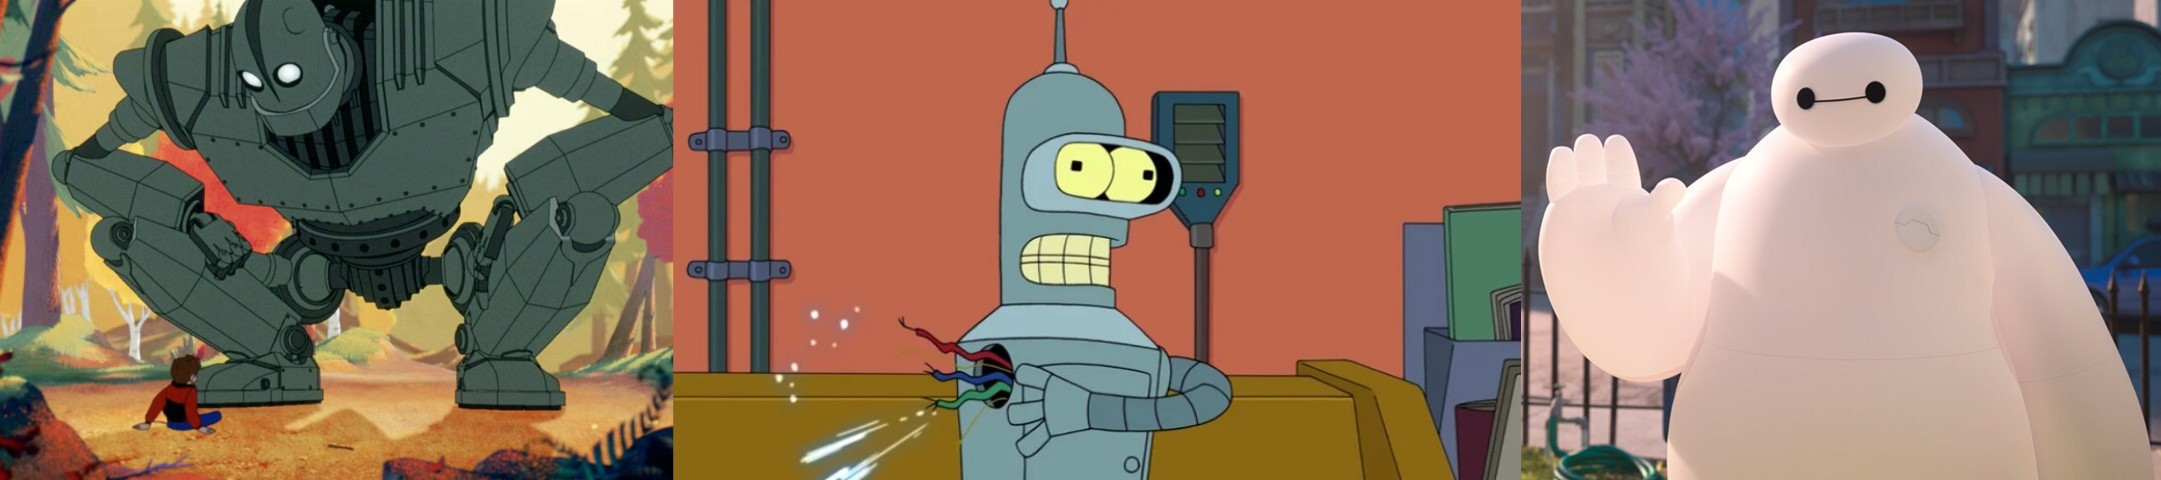
\includegraphics[width=\textwidth]{figures/01-introduction/robots-in-animation.jpg}
    \caption{The Iron Giant \cite{TheIronGiant1999}.
        Bender Futurama \cite{Futurama1999}.
        Baymax Big Hero 6 \cite{BigHero62014}.
    }
    \label{fig:introduction:robots-in-animation}
\end{figure}

\begin{figure}
    \centering
    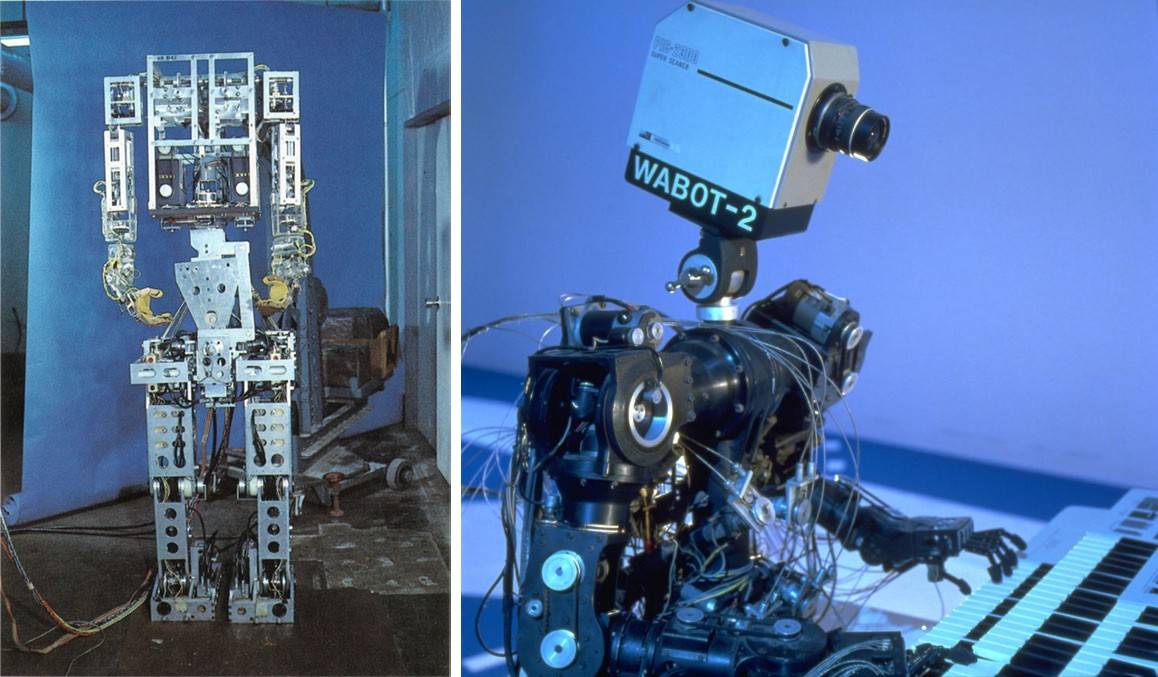
\includegraphics[width=0.7\textwidth]{figures/01-introduction/WABOTs.jpg}
    \caption{WABOT-1 \cite{Kato1973TheWABOT1}. WABOT-2 \cite{Kato1987WABOT2}.}
    \label{fig:introduction:WABOTs}
\end{figure}

\begin{figure}
    \centering
    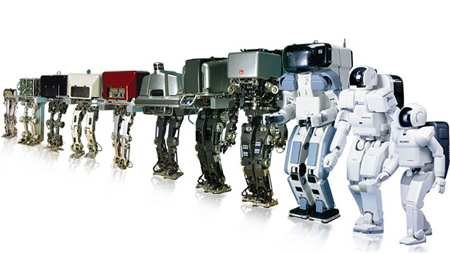
\includegraphics[width=0.7\textwidth]{figures/01-introduction/The-ASIMO-humanoid-robot-history.png}
    \caption{From Honda E0 to ASIMO \cite{Shigemi2019ASIMOandHumanoidRobotResearchatHonda}.}
    \label{fig:introduction:ASIMO-humanoid-history}
\end{figure}

\begin{figure}
    \centering
    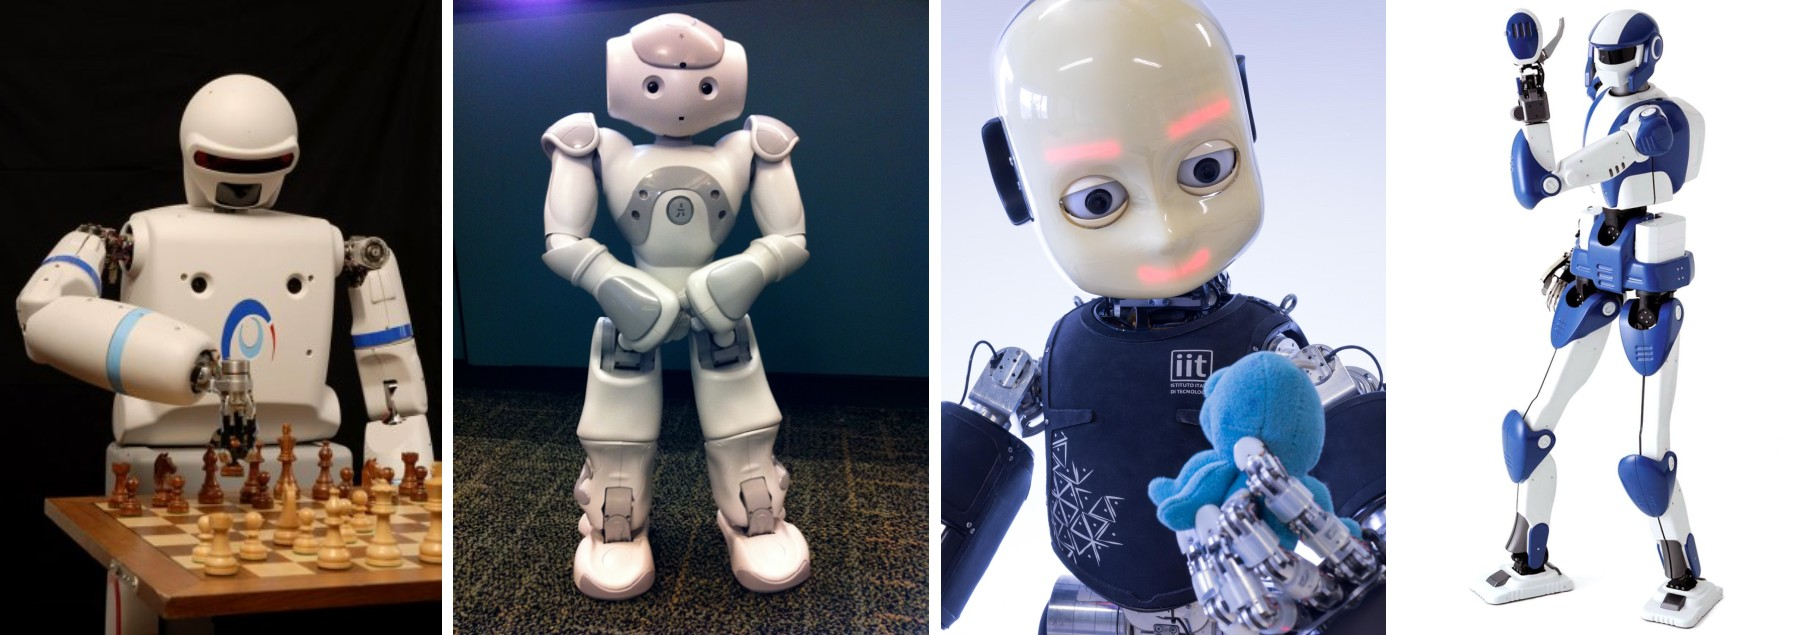
\includegraphics[width=\textwidth]{figures/01-introduction/robots-in-2000.jpg}
    \caption{PAL Robotics REEM-B \cite{Tellez2008REEMB}.
        Aldebaran NAO \cite{Gouaillier2008NAOHumanoid}.
        iCub \cite{Metta2010iCubHumanoid}.
        HRP-4 \cite{Kaneko2011HRP4}.
    }
    \label{fig:introduction:robots-in-2000}
\end{figure}

\begin{figure}
    \centering
    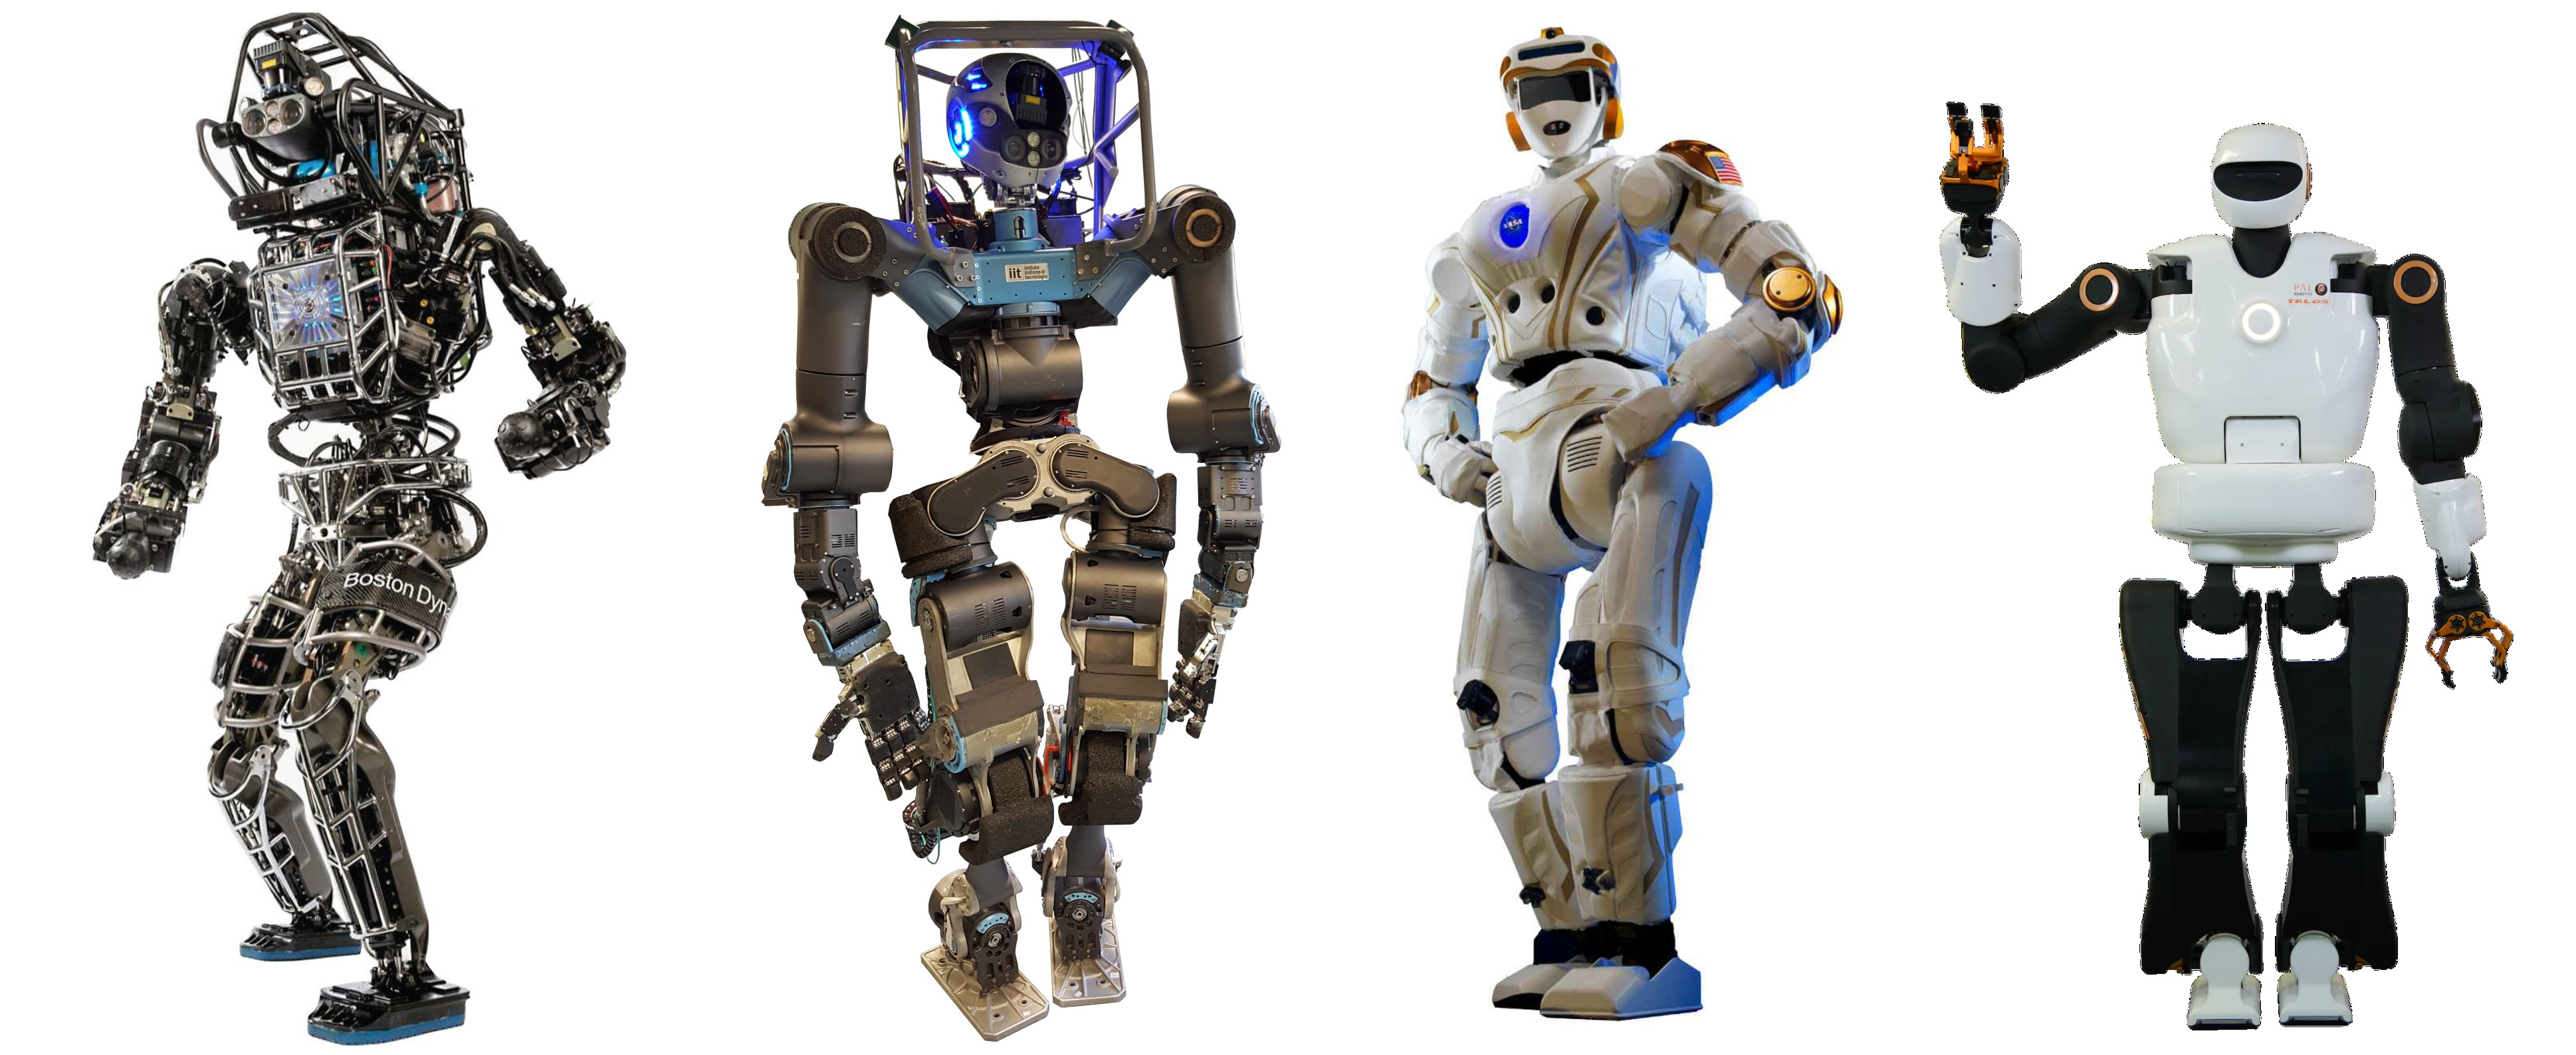
\includegraphics[width=\textwidth]{figures/01-introduction/robots-in-2010.jpg}
    \caption{Boston Dynamics ATLAS. WALK-MAN \cite{Tsagarakis2017WALKMAN}.
        NASA Valkyrie \cite{Radford2015Valkyrie}.
        PAL Robotics TALOS \cite{Stasse2017TALOS}.}
    \label{fig:introduction:robots-in-2010}
\end{figure}

\begin{figure}
    \centering
    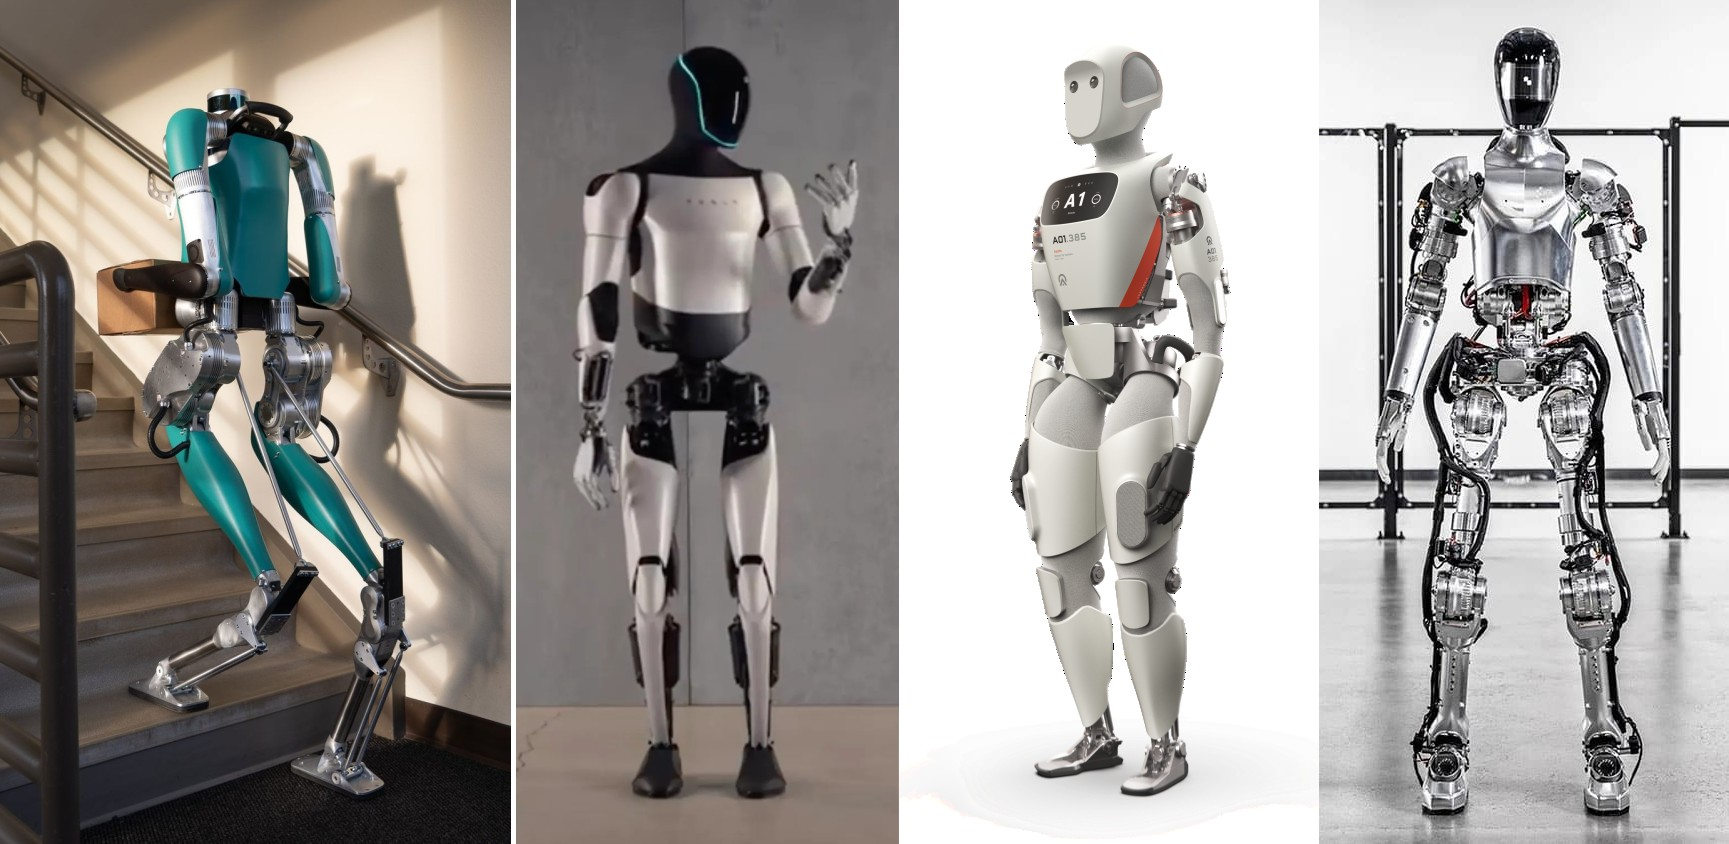
\includegraphics[width=\textwidth]{figures/01-introduction/robots-in-2020.jpg}
    \caption{Digit by Agility Robotics. Optimus by Tesla. Apollo by Apptronik.
        Figure 01 by Figure AI.
    }
    \label{fig:introduction:robots-in-2020}
\end{figure}

\begin{figure}
    \centering
    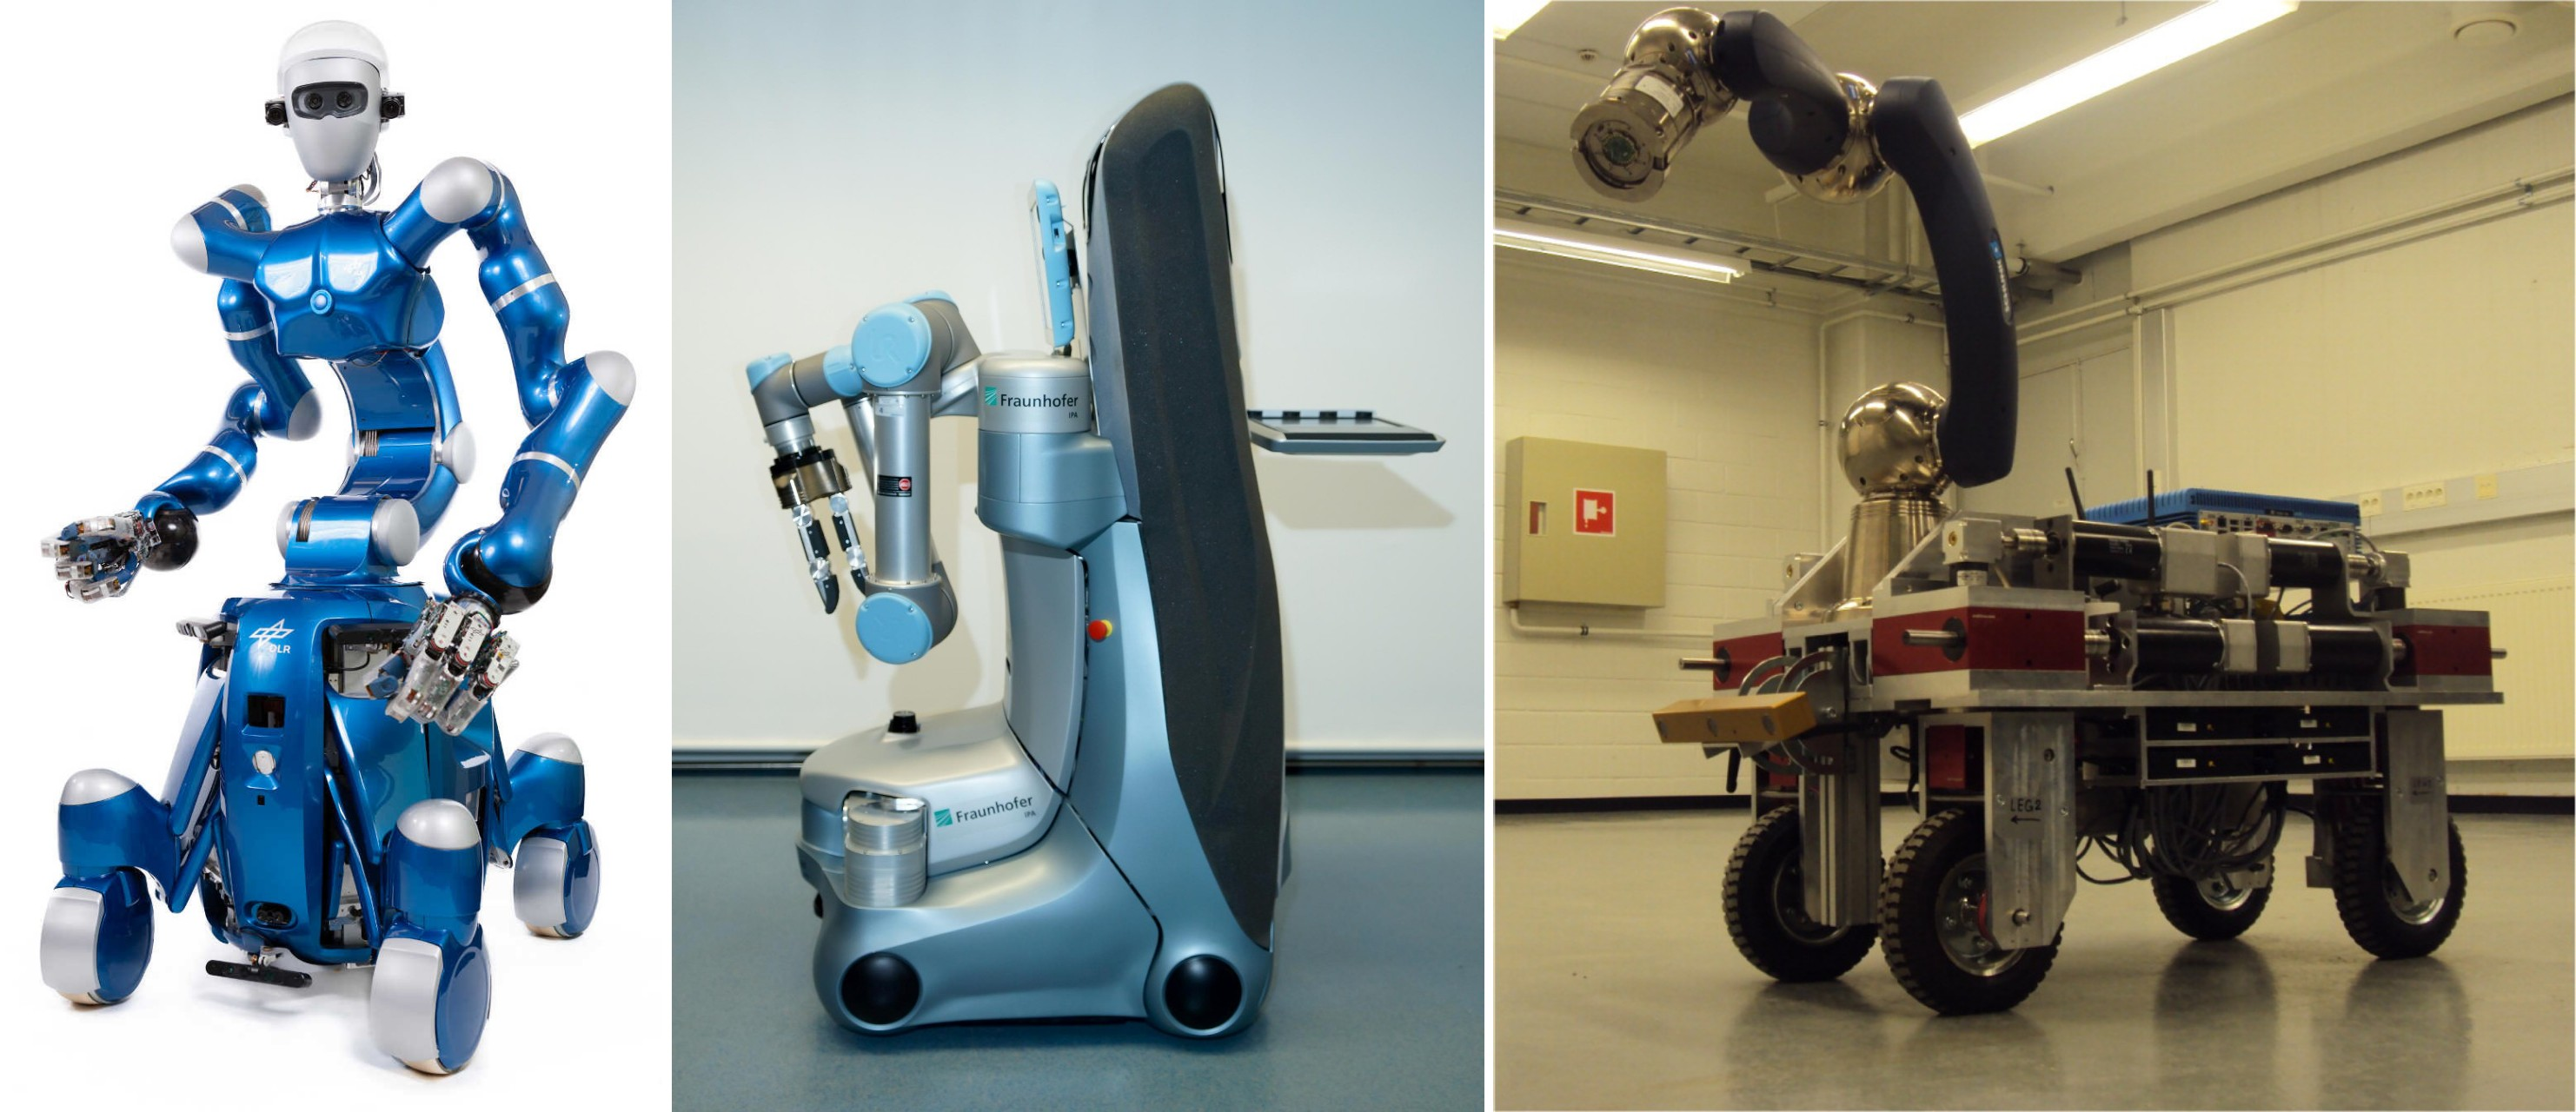
\includegraphics[width=\textwidth]{figures/01-introduction/SWMRs-1.jpg}
    \caption{Rollin' Justin \cite{Fuchs2009RollinJustin}.
        Care-O-bot 3 \cite{Graf2009Care-O-bot3}.
        iMoro \cite{Oftadeh2013iMoro}.}
    \label{fig:introduction:SWMRs-1}
\end{figure}

\begin{figure}
    \centering
    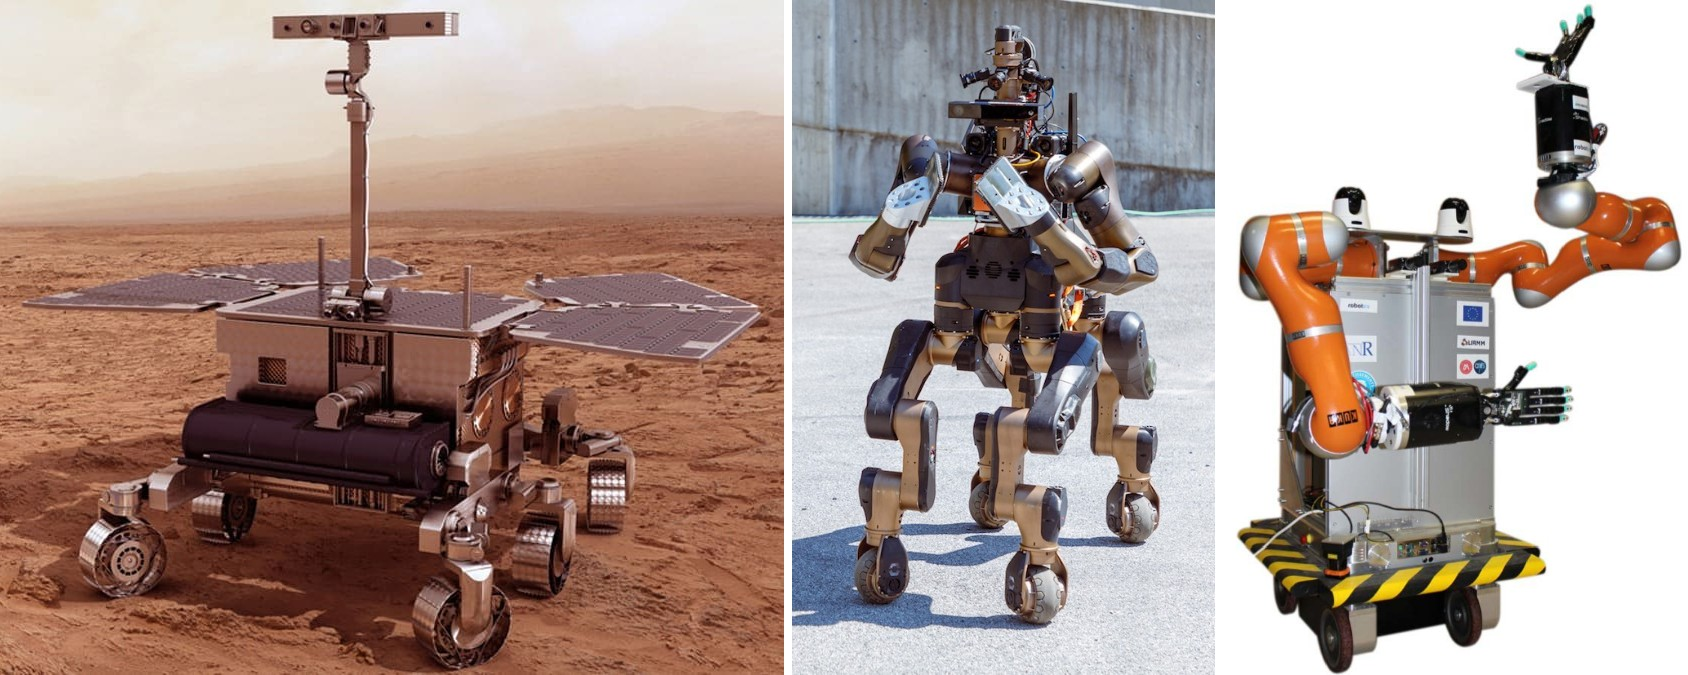
\includegraphics[width=\textwidth]{figures/01-introduction/SWMRs-2.jpg}
    \caption{ExoMars \cite{Poulakis2015ExoMarsMobilitySubsystem}.
        CENTAURO \cite{Kashiri2019Centauro}.
        BAZAR \cite{Cherubini2019ACR}.
    }
    \label{fig:introduction:SWMRs-2}
\end{figure}


\section{Contribution}
Thesis contribution and list of publications.

\section{Outline}
Outline of the thesis.
